\documentclass[10pt,letterpaper]{article}
\usepackage[utf8]{inputenc}
\usepackage{amsmath}
\usepackage{amsfonts}
\usepackage{amssymb}
\usepackage{graphicx}
\usepackage[left=1.5cm,right=1.5cm,top=1cm,bottom=1cm]{geometry}
\title{Hints on lmcholsolve}
\author{yifan}

\begin{document}
\maketitle
lmcholsolve in optimise2 will solve the following question using Cholesky-decomposition:
\begin{equation}
H\beta=y\quad H>0
\end{equation}
It is a little bit tricky to compare the performances of \textit{base::solve} and \textit{optimise2::lmcholsolve}. The original \textit{solve} used in R relies on the BLAS you choose. On my Mac machine, I use vecBLAS and openBLAS with MacPro1,1(2 X Intel(R) Xeon(R) CPU  X5355   2.66GHz), the performances are shown in Fig[\ref{perf}].
\begin{figure}[ht]
\centering
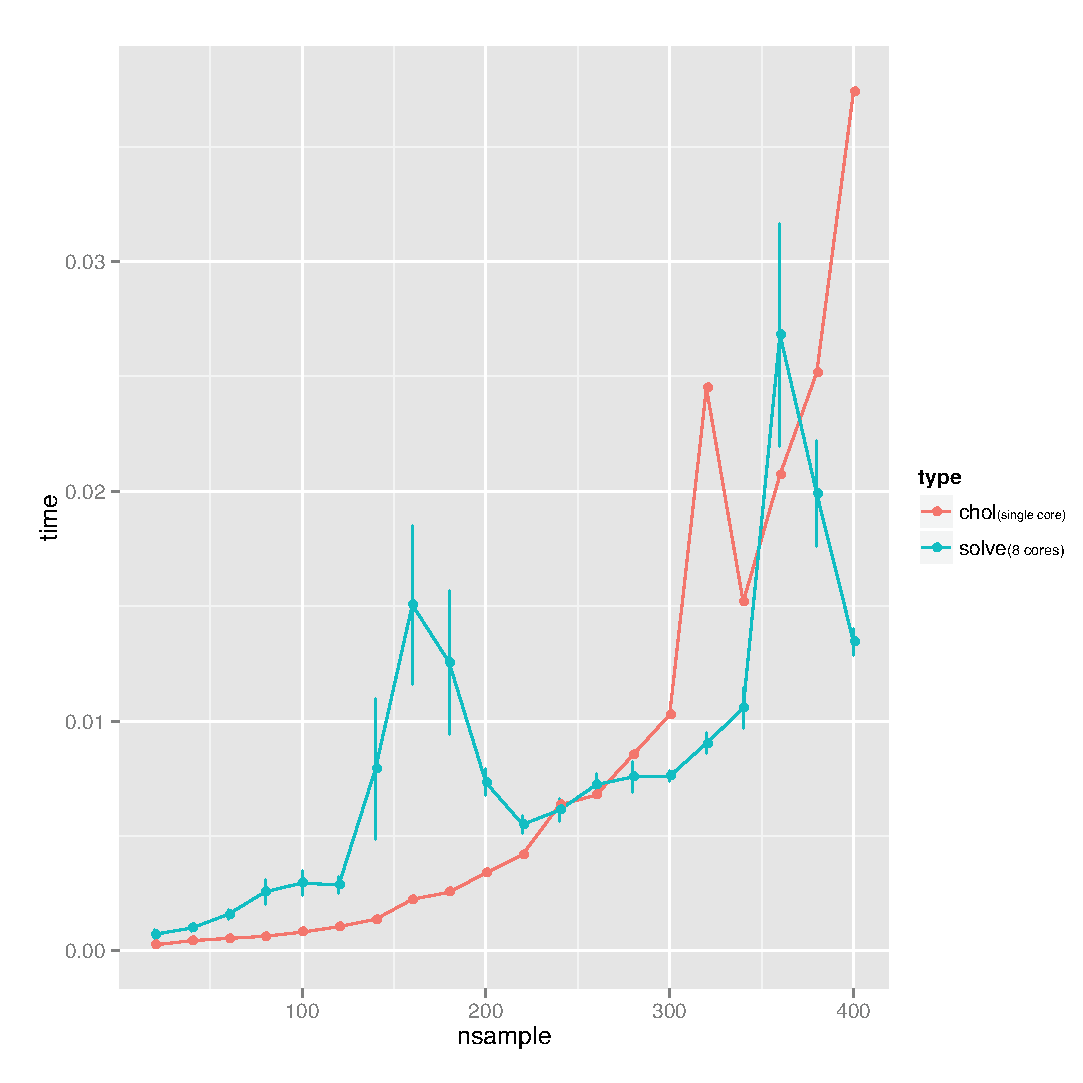
\includegraphics[scale=.6]{perf.eps}
\caption{100 simulation.}\label{perf}
\end{figure}
\noindent{}Although \textit{solve} uses all 8 cores \footnote{In fact , it should be 4 cores 8 threads}, \textit{optimise2::lmcholsolve} is still not so bad when sample size is less than 300.  Parallel QR-decomposition/householder transformation may boost the solution, but it is not of my concern now. One thing I must state is the function will not check the following conditions are true or not:
\begin{itemize}
\item[1] $H\geq 0$ (or even it is a square matrix);
\item[2] the dimensions of $H$ and $y$ agree with each other.
\end{itemize}

In \textbf{serious} studies, one may use $svd$ instead of sweeping/householder/QR as $svd$ tends to do a better job than others in the sense of accuracy and stability. The weakness of svd is speed. Generally speaking, if the design matrix is nearly singular, sweeping, which is used is SAS, performs the worst among all.

\end{document}